\documentclass[a4paper, 12pt]{article}
\usepackage{caption}
\usepackage{graphicx}
\graphicspath{{images/}}
\usepackage{listings}
\usepackage[english]{babel}
\usepackage{caption}
\usepackage{color}
\usepackage{array}

\title{Homework 2}
\author{Nasir Mohammad Khalid}

\makeatletter
\let\thetitle\@title
\let\theauthor\@author
\let\thedate\@date
\makeatother

\definecolor{codegreen}{rgb}{0,0.6,0}
\definecolor{codegray}{rgb}{0.5,0.5,0.5}
\definecolor{codepurple}{rgb}{0.58,0,0.82}
\definecolor{backcolour}{rgb}{0.95,0.95,0.92}

\lstdefinestyle{mystyle}{
    backgroundcolor=\color{backcolour},   
    commentstyle=\color{codegreen},
    keywordstyle=\color{magenta},
    numberstyle=\tiny\color{codegray},
    stringstyle=\color{codepurple},
    basicstyle=\scriptsize,
    breakatwhitespace=false,         
    breaklines=true,                 
    captionpos=b,                    
    keepspaces=true,                 
    numbers=left,                    
    numbersep=1pt,                  
    showspaces=false,                
    showstringspaces=false,
    showtabs=false,                  
    tabsize=1
}

\lstset{style=mystyle}

\newenvironment{conditions}
  {\par\vspace{\abovedisplayskip}\noindent\begin{tabular}{>{$}l<{$} @{${}={}$} l}}
  {\end{tabular}\par\vspace{\belowdisplayskip}}

\begin{document} 
    \begin{titlepage}
        \centering
        \vspace*{0.5 cm}
        
\includegraphics[scale = 0.60]{logo.png}\\[1.0 cm]	% University Logo
        \textsc{\LARGE American University of Sharjah}\\[1.0 cm]
        \textsc{\Large ELE494-09}\\[0.2 cm]	
        \textsc{\Large Deep Networks in Machine Learning}\\[0.5 cm]			% Course Code
        \rule{\linewidth}{0.2 mm} \\[0.4 cm]
        { \huge \bfseries \thetitle}\\
        \rule{\linewidth}{0.2 mm} \\[1.5 cm]
        
        \textsc{\Large{\theauthor}}\\[0.3 cm]
        \textsc{\Large{65082}}\\[0.3 cm]
        \textsc{\Large{\thedate}}\\[1.5 cm]

        \textmd{Submitted To: \itshape{Dr.Usman Tariq}}
    \end{titlepage}

    \clearpage
    \tableofcontents
    \listoffigures
    \lstlistoflistings
    \clearpage

    \section{Task 1: Backpropagation}

    \subsection{Q1.1}

    The goal of this part to develop a theoretical understanding of how do you get the expressions with
    backpropagation algorithm. Suppose you have a three layer fully connected neural network (input layer,
    hidden layer and output layer). Following are some further "specifications":

    \begin{itemize}
        \item The input feature vectors are d dimensional (you can think of these as MNIST images, attened as vectors)
        \item There are N feature vectors in you training dataset
        \item There are H hidden nodes and K output nodes (for K mutually exclusive classes).
        \item This neural network is to be trained for classification under cross-entropy loss function
    \end{itemize}

    Derive the equations for batch gradient updates for the input-to-hidden unit weights and hidden-to-output
    unit weights. Is it wise to use a learning rate parameter? Why?

    \subsection{Background to Answer}
    
    Based on the specifications given we can assume the architecture of the neural network to be as follows:

    \begin{figure}[h!]
        \centering
        \captionsetup{justification=centering}
        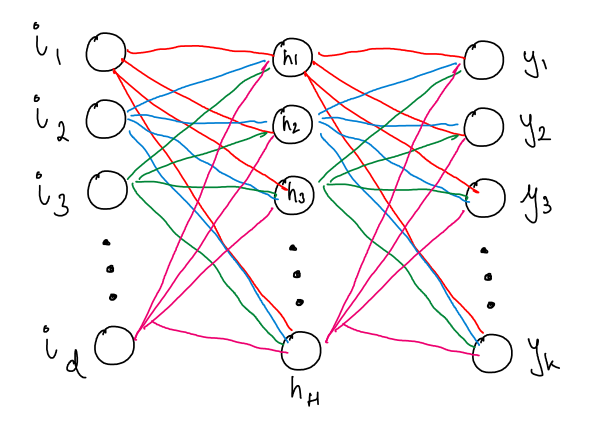
\includegraphics[scale = 0.37]{1.png}
        \caption{Representation of the neural network}
    \end{figure}
    
    The output of the node 'h' of hidden layer will be calculated using the sigmoid activation function and is given as follows:

    \begin{equation}
        Z_h = \sum_{n=1}^{d} i_n * w_{nh} + b_h
    \end{equation}

    \begin{equation}
        O_h = \frac{1}{1+e^{Z_h}}
    \end{equation}

    \begin{center}
        \begin{conditions}
            $$Z_h$$     &   Input to the sigmoid function of node 'h' \\
            $$O_h$$     &   Output of the sigmoid function of the node 'h' \\   
            $$b_h$$     &   Bias of the input to node h \\   
            $$w_{nh}$$  &   Weight between input node $$n$$ and the hidden node $$h$$\\
        \end{conditions}
    \end{center}
    
    The output of the node 'o' of the final layer will be calculated using the softmax function and it will be given as follows:
    
    \begin{equation}
        Z_o = \sum_{n=1}^{h} O_{n} * w_{no} + b_o
    \end{equation}

    \begin{equation}
        Y_o = \frac{e^{Z_o}} {\sum_{j=1}^{k} e^{Z_j}}
    \end{equation}

    \begin{center}
        \begin{conditions}
            $$Z_o$$     &   Input to the softmax function of node 'o' \\
            $$Y_o$$     &   Output of the 'o'th output layer \\
            $$b_o$$     &   Bias of the Output node 'o' \\
            $$w_{no}$$  &   Weight between the 'n'th hidden node to the 'o'th output node\\
        \end{conditions}
    \end{center}

    The output layer will give values between 0 and 1 only. The error function is the cross-entropy function. Since the output consists of K mutually exclusive classes then we can take the label for the feature vectors to be of a matrix of length K
    and it contains a 1 at the appropriate label. Then the cross entropy loss function is given as:

    \begin{equation}
        E = - \sum_{i=1}^{k} L_i * log(Y_i)
    \end{equation}
    \begin{center}
        \begin{conditions}
            $$E$$       &   Error value from the cross-entropy function \\
            $$L_k$$     &   Value of the label at the 'k'th index \\   
            $$Y_k$$     &   Output of output node 'k'\\
        \end{conditions}
    \end{center}

    Now we want to get the derivative of the error with respect to the first set of weights between the hidden layer and output layer:

    \begin{equation}
        \frac{\partial E}{\partial w_{hk}} = \frac{\partial E}{\partial Z_k} * \frac{\partial Z_k}{\partial w_{hk}}
    \end{equation}

    \begin{center}
        \begin{conditions}
            $$\frac{\partial E}{\partial w_{hk}}$$      &   $\partial$ of Error function w.r.t weights between hidden and output layer \\[0.3 cm]
            $$\frac{\partial E}{\partial Z_k}$$         &   $\partial$ of the Error function with respect to the input to the softmax\\[0.3 cm]
            $$\frac{\partial Z_k}{\partial w_{hk}}$$    &   $\partial$ of input to softmax w.r.t  weights between hidden and output layer\\[0.3 cm]
        \end{conditions}
    \end{center}

    The derivative of the softmax function $Y_o$ with respect to the input of the softmax function $Z_k$ is obtained through the quotient rule and is given by:
    
    \begin{equation}
        \frac{\partial Y_o}{\partial Z_k} = Y_k * (1-Y_j) = Y_k * (1-Y_k) \quad {when \quad j = k}
    \end{equation}

    \begin{equation}
        \frac{\partial Y_o}{\partial Z_k} = - Y_j * Y_k \quad {when \quad j \neq k}
    \end{equation}\\

    The derivative of the error with respect to the input to the softmax can will consist of two parts. The first is when $i = k$ (in summation) and the second is when they are not the same:

    \begin{equation}
        \frac{\partial E}{\partial Z_k} = - \sum_{i=1}^{k} L_i * \frac{\partial log(Y_i)}{\partial Y_i} * \frac{\partial Y_i}{\partial Z_k} 
    \end{equation}

    \begin{equation}
        \frac{\partial E}{\partial Z_k} = -L_k * \frac{\partial log(Y_k)}{\partial Y_k} * \frac{\partial Y_k}{\partial Z_k} = -L_k * (1-Y_j) \quad {when \quad i = k}
    \end{equation}

    \begin{equation}
        \frac{\partial E}{\partial Z_k} = - \sum_{i \neq k} L_i * \frac{\partial log(Y_i)}{\partial Y_i} * \frac{\partial Y_i}{\partial Z_k} =  \sum_{i \neq k} L_i * Y_j \quad {when \quad i \neq k}
    \end{equation}

    We take the summation of both cases to get the final derivative of error with respect to the input to the softmax function:

    \begin{equation}
        \frac{\partial E}{\partial Z_k} = -L_k * (1-Y_j) + \sum_{i \neq k} L_i * Y_j
    \end{equation}
    
    \begin{equation}
        \frac{\partial E}{\partial Z_k} = Y_j * (L_k + \sum_{i \neq k} L_i) - L_k
    \end{equation}
    
    but $(L_k + \sum_{i \neq k} L_i)$ is equal to 1 as it is all the intended outputs added up. Due to the fact that the outputs are always probabilities their sum will give 1 and therefore we get the final expression:

    \begin{equation}
        \frac{\partial E}{\partial Z_k} = Y_j - L_k = Y_k - L_k
    \end{equation} 

    \begin{center}
        \begin{conditions}
            $$\frac{\partial E}{\partial Z_k}$$      &   $\partial$ of Error function w.r.t input to the softmax function \\[0.3 cm]
            $$Y_k$$                                  &   It is the final output of the output neuron\\[0.3 cm]
            $$L_k$$                                  &   It is the intended output of the output neuron \\[0.3 cm]
        \end{conditions}
    \end{center}

    Similarly we the derivative of the input to the softmax with respect to the weights. Here $O_h$ is the output of the hidden layer:

    \begin{equation}
        \frac{\partial Z_k}{\partial w_{hk}} = O_h
    \end{equation}

    \subsection{A1: Gradient Update for hidden-to-output weights}

    The final answer is given by: 

    \begin{equation}
        \frac{\partial E}{\partial w_{hk}} = \frac{\partial E}{\partial Z_k} * \frac{\partial Z_k}{\partial w_{hk}} = (Y_k - L_k) * O_h
    \end{equation}
    
    \begin{center}
        \begin{conditions}
            $$\frac{\partial E}{\partial w_{hk}}$$   &   $\partial$ of Error function w.r.t weights between hidden-output \\[0.3 cm]
            $$Y_k$$                                  &   It is the final output of the output neuron\\[0.3 cm]
            $$L_k$$                                  &   It is the intended output of the output neuron \\[0.3 cm]
            $$O_h$$                                  &   It is the final output of the hidden neuron\\[0.3 cm]
        \end{conditions}
    \end{center}
    
    \subsection{A2: Gradient Update for input-to-hidden weights}

    Here we further extend the partial derivatives until we get the change in error with respect to the input-hidden weights. Since the output of one hidden layer neuron is sent all output neurons we take a summation over all output neurons. 
    \begin{equation}
        \frac{\partial E}{\partial w_{ih}} = \sum_{b=1}^{k} \frac{\partial E}{\partial Z_b} * \frac{\partial Z_b}{\partial O_h} * \frac{\partial O_h}{\partial Z_h} * \frac{\partial Z_h}{\partial w_{ih}}
    \end{equation}

    \begin{center}
        \begin{conditions}
            $$\frac{\partial E}{\partial w_{ih}}$$   &   $\partial$ of Error function w.r.t weights between input-hidden \\[0.3 cm]
            $$\frac{\partial E}{\partial Z_b}$$      &   $\partial$ of Error function w.r.t input to softmax for neuron b \\[0.3 cm]
            $$\frac{\partial Z_b}{\partial O_h}$$    &   $\partial$ of Input to softmax for neuron b w.r.t output of hidden \\[0.3 cm]
            $$\frac{\partial O_h}{\partial Z_h}$$    &   $\partial$ of Output of hidden w.r.t input to sigmoid\\[0.3 cm]
            $$\frac{\partial Z_h}{\partial w_{ih}}$$ &   $\partial$ of Input to sigmoid w.r.t weight between input and hidden \\[0.3 cm]
        \end{conditions}
    \end{center}

    We already obtained the first term $ \frac{\partial E}{\partial Z_b} $ in section 1.4 and the rest are derived below. The first one (18) where $w_{hb}$ is the weight between hidden neuron h and output neuron b

    \begin{equation}
        \frac{\partial Z_b}{\partial O_h} = w_{hb}
    \end{equation}

    (19) is derivative of the sigmoid function

    \begin{equation}
        \frac{\partial O_h}{\partial Z_h} = O_h * (1- O_h)
    \end{equation}

    Here $ i_n $ is the input to the network

    \begin{equation}
        \frac{\partial Z_h}{\partial w_{ih}} = i_n
    \end{equation}

    Combining all of these together gives the final equation for the change in error with respect to the weights between input-hidden layer.

    \begin{equation}
        \frac{\partial E}{\partial w_{ih}} = \sum_{b=1}^{k} (Y_b - L_b) * w_{hb} * O_h * (1-O_h) * i_n
    \end{equation}

    \begin{center}
        \begin{conditions}
            $$\frac{\partial E}{\partial w_{ih}}$$   &   $\partial$ of Error function w.r.t weights between input-hidden \\[0.3 cm]
            $$Y_b$$                                  &   Output of the final neuron 'b'\\[0.3 cm]
            $$L_b$$                                  &   Intended output of final neuron 'b'\\[0.3 cm]
            $$w_{hb}$$                               &   Weights between hidden neuron 'h' and output neuron 'b'\\[0.3 cm]
            $$O_h$$                                  &   Output of hidden neuron\\[0.3 cm]
            $$i_n$$                                  &   Input of first neuron\\[0.3 cm]
        \end{conditions}
    \end{center}

    \subsection{A3: Learning Parameter}

    In this situation using a learning parameter would be useful because for the backpropagation in equation (21) if the input $i_n$ is a large value
    then the weights would not update by a small value. Since we are using the MNIST database the values could range from 0-255

    \section{Task 2: Implementation}

    \subsection{Q2}

    Import the Fashion mnist dataset then divide the training images further, into 40,000 training and 20,000 validation images. Make sure you do this at random. So now you will have 40,000 training images, 20,000 validation images and 10,000 testing images. 
    
    \begin{itemize}
        \item Read about the fashion mnist dataset and report the highlights (e.g. number of images, number of classes etc) along with some example images.
        \item What will be reasonable loss function to use for classification if the last layer activation functions are soft-max functions? Explain your rationale.
        \item Train four neural networks each with one hidden layer; one with 16 nodes, one with 64 nodes, one with 128 node and one with 512 nodes. Train each one of them for 15 epochs.
        \begin{itemize}
            \item Which one of them gives you the best performance on the validation data?
            \item Does increasing epoch to 30 improve the validation performance?
            \item Experiment with using sigmoid and relu as activation functions for the hidden layer. Plot the validation loss or validation accuracy for both kinds of activation functions for all the four network models against the number of epochs (30). This will give you 8 plots. Comment on the plots and comparison across the choice of activation functions
            \item Pick the model parameters that give you the best performance, then combine your validation data with training data, retrain your network with optimum parameters and report the classification accuracy as well as the confusion matrix on the test data
        \end{itemize}
    \end{itemize}
    
    \subsection{A1: Fashion-MNIST Details}

    Fashion-MNIST is a dataset consisting of different articles of clothing. It has a training set of 60,000 examples and a test set of 10,000 examples. Each example is a 28x28 grayscale image, associated with a label from 10 classes. Below is an image of the entire Fasion MNIST dataset

    \begin{figure}[h!]
        \centering
        \captionsetup{justification=centering}
        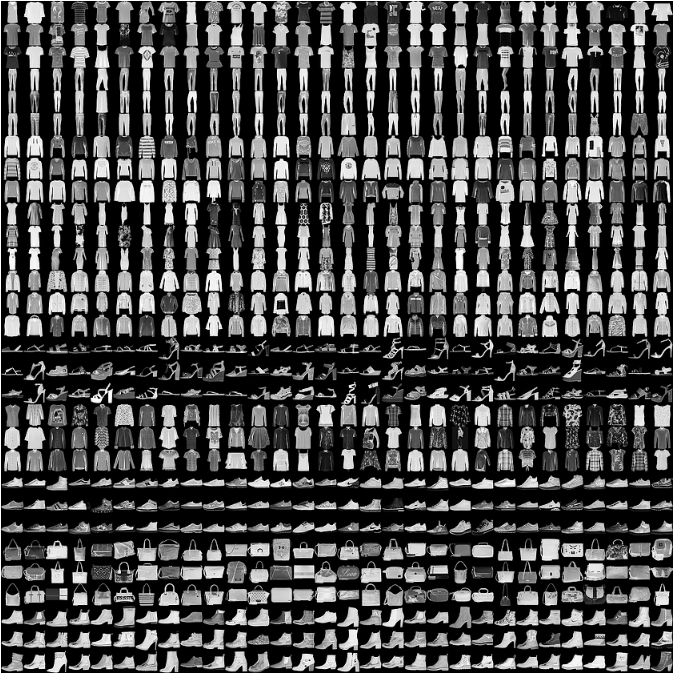
\includegraphics[scale = 0.37]{2.png}
        \caption{Fashion MNIST Dataset Images}
    \end{figure}

    \subsection{A2: Reasonable Loss Function}

    If the last layer has a softmax output, this means that each neuron would output a probability between 0 and 1. The sum of the last layer activations would be 1. The reasonable loss function would be the cross-entropy loss because it has a large gradient when the output value is far from 1 and as the output becomes 1 the gradient changes slowly therefore preventing overshooting the minima. The cross entropy works best for probabilities and helps speed up learning.

    Furthermore, the softmax ensures that no two classes are returned simultaneously since it returns the probability for each class.
    
    \subsection{A3: Training 4 Neural Networks}

    The code used to train the 4 networks is included in the python notebook. Outlined here are the results of the 4 training cases.
    
    \subsubsection{16 nodes and 15 epochs}

    This was the best performing network. The final training data accuracy was 0.8648

    \begin{figure}[h!]
        \centering
        \captionsetup{justification=centering}
        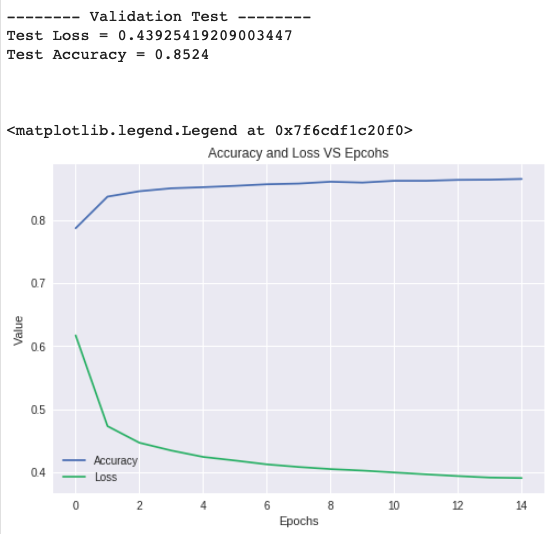
\includegraphics[scale = 0.37]{16_15.png}
        \caption{Trained with 16 hidden nodes and 15 epochs}
    \end{figure}

    \subsubsection{64 nodes and 15 epochs}

    The final training data accuracy was 0.8620

    \begin{figure}[h!]
        \centering
        \captionsetup{justification=centering}
        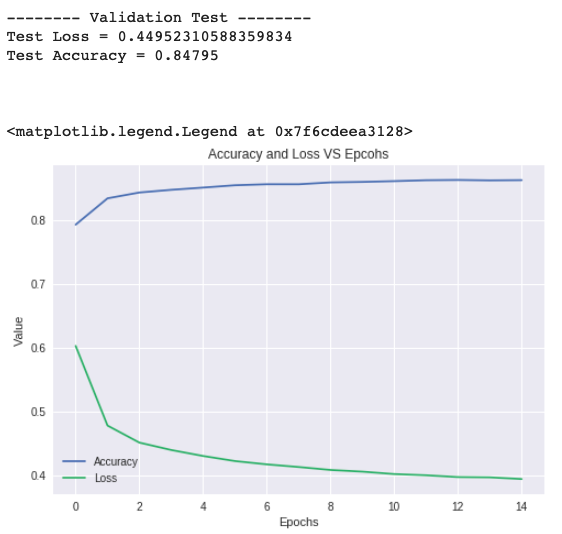
\includegraphics[scale = 0.37]{64_15.png}
        \caption{Trained with 64 hidden nodes and 15 epochs}
    \end{figure}
    
    \subsubsection{128 nodes and 15 epochs}

    The final training data accuracy was 0.8603

    \begin{figure}[h!]
        \centering
        \captionsetup{justification=centering}
        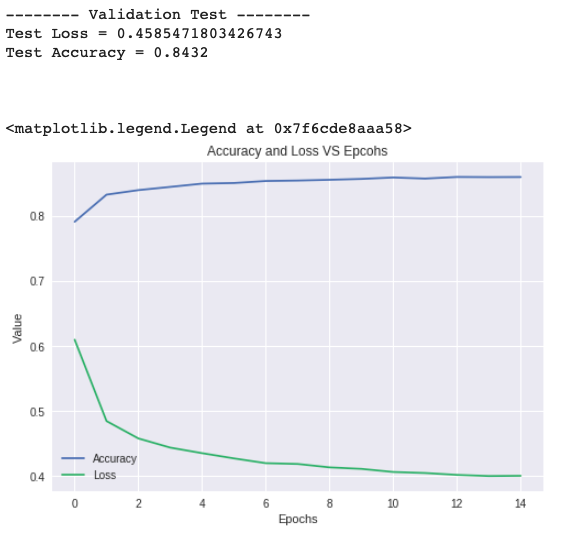
\includegraphics[scale = 0.37]{128_15.png}
        \caption{Trained with 128 hidden nodes and 15 epochs}
    \end{figure}

    \subsubsection{512 nodes and 15 epochs}

    The final training data accuracy was 0.8567
    
    \begin{figure}[h!]
        \centering
        \captionsetup{justification=centering}
        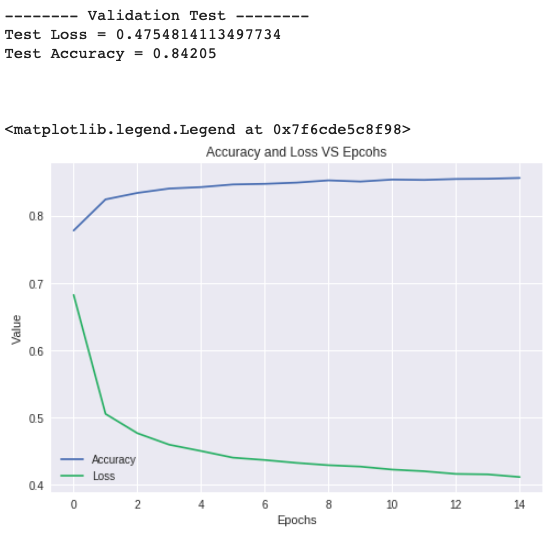
\includegraphics[scale = 0.37]{512_15.png}
        \caption{Trained with 512 hidden nodes and 15 epochs}
    \end{figure}

    \subsection{A4: Increasing the epochs to 30}

    The jupyter notebook shows the code used and the changes from moving to 30 epochs. Overall, if there is a large number of neurons then the validation performance increases at 30 epochs. For a small number of neurons, increasing the epochs made it worse.


    \subsubsection{For 16 Neurons}
    
    The test accuracy decreased by 0.00225. The test loss increased by 0.004325. For 16 neurons it did not really improve the validation performance.

    \subsubsection{For 64 Neurons}

    The test accuracy decreased by 0.0086. The test loss increased by 0.033835. For 64 neurons it did not really improve the validation performance.

    \subsubsection{For 128 Neurons}

    The test accuracy increased by 0.00475. The test loss decreased by 0.006488. For 32 neurons it improved the validation performance.

    \subsubsection{For 512 Neurons}

    The test accuracy increased by 0.0073. The test loss decreased by 0.025331. For 512 neurons it improved the validation performance.

    \subsection{A5: Hidden Layer Activation Function}

    The code for different neurons and activation functions is included in the jupyter notebook. Below are the results for different neurons and activations each with 30 epochs

    \subsubsection{For 16 Neurons}

    Here the sigmoid activation performed better even though it started with a very high loss function value. Below is the RELU activation

    \begin{figure}[h!]
        \centering
        \captionsetup{justification=centering}
        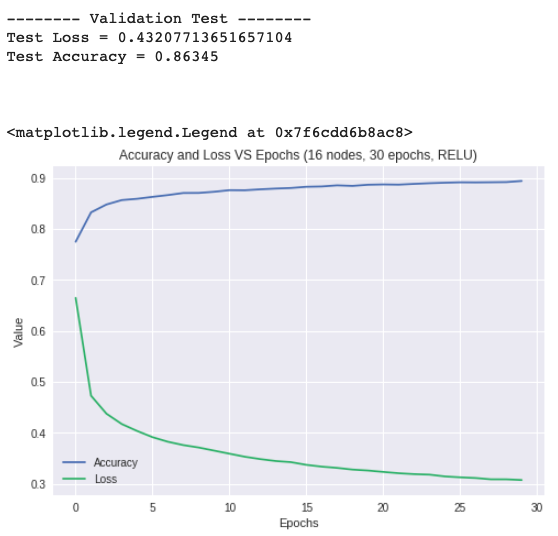
\includegraphics[scale = 0.3]{16_RELU.png}
        \caption{16 Neurons and RELU}
    \end{figure}

    Below is the Sigmoid activation
    
    \begin{figure}[h!]
        \centering
        \captionsetup{justification=centering}
        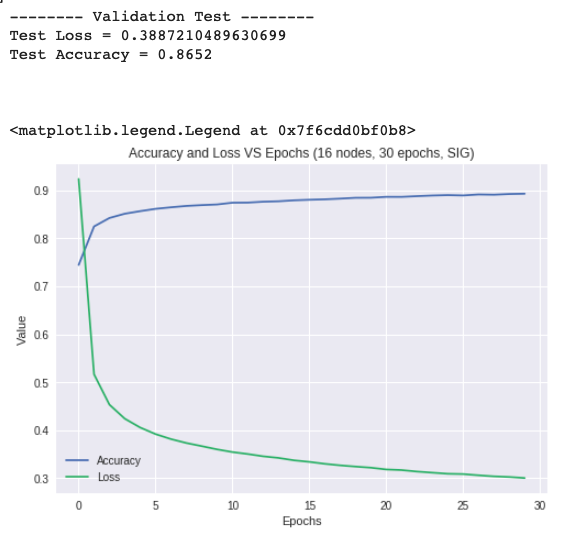
\includegraphics[scale = 0.3]{16_SIG.png}
        \caption{16 Neurons and Sigmoid}
    \end{figure}

    \subsubsection{For 64 Neurons}

    Here the sigmoid activation performed better. Below is the RELU activation

    \begin{figure}[h!]
        \centering
        \captionsetup{justification=centering}
        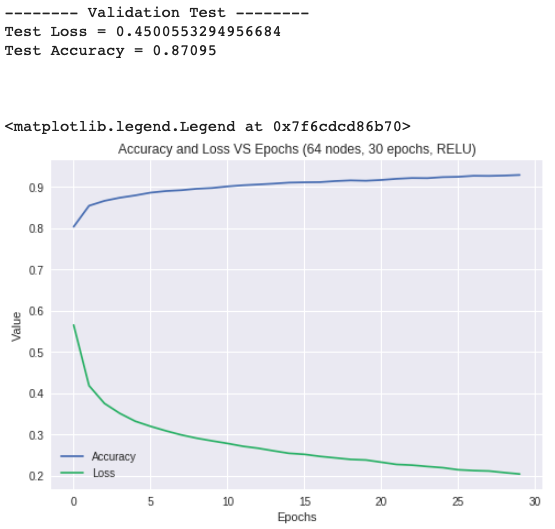
\includegraphics[scale = 0.3]{64_RELU.png}
        \caption{64 Neurons and RELU}
    \end{figure}

    Below is the Sigmoid activation
    
    \begin{figure}[h!]
        \centering
        \captionsetup{justification=centering}
        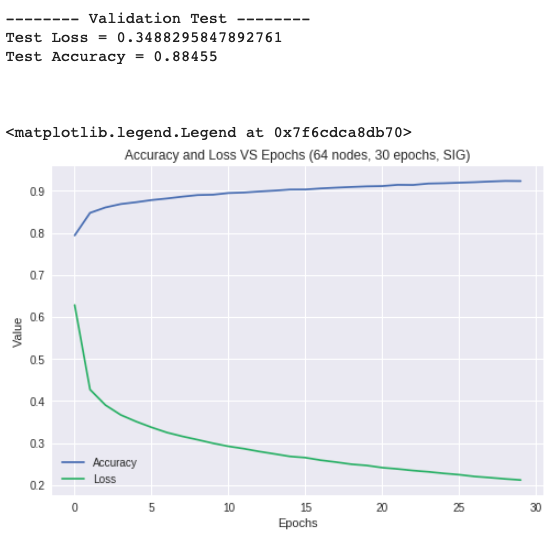
\includegraphics[scale = 0.3]{64_SIG.png}
        \caption{64 Neurons and Sigmoid}
    \end{figure}

    \pagebreak
    \subsubsection{For 128 Neurons}

    Here the sigmoid activation performed better. Below is the RELU activation

    \begin{figure}[h!]
        \centering
        \captionsetup{justification=centering}
        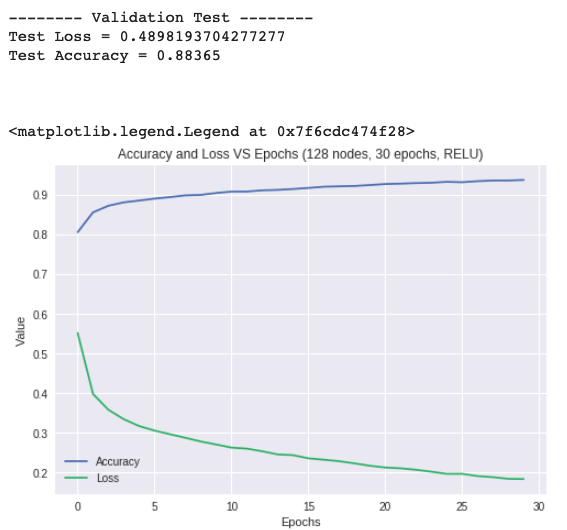
\includegraphics[scale = 0.3]{128_RELU.png}
        \caption{128 Neurons and RELU}
    \end{figure}

    Below is the Sigmoid activation
    
    \begin{figure}[h!]
        \centering
        \captionsetup{justification=centering}
        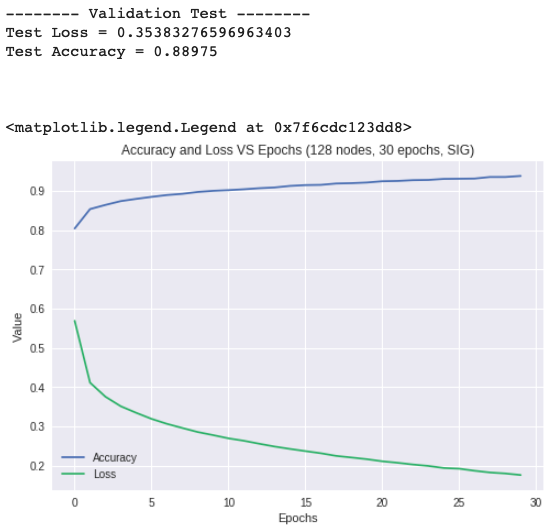
\includegraphics[scale = 0.3]{128_SIG.png}
        \caption{128 Neurons and Sigmoid}
    \end{figure}

    \pagebreak
    \subsubsection{For 512 Neurons}

    Here the sigmoid activation performed better. Below is the RELU activation

    \begin{figure}[h!]
        \centering
        \captionsetup{justification=centering}
        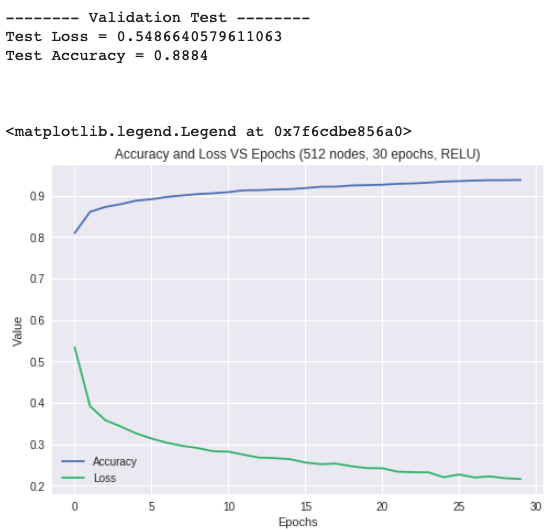
\includegraphics[scale = 0.3]{512_RELU.png}
        \caption{512 Neurons and RELU}
    \end{figure}

    Below is the Sigmoid activation
    
    \begin{figure}[h!]
        \centering
        \captionsetup{justification=centering}
        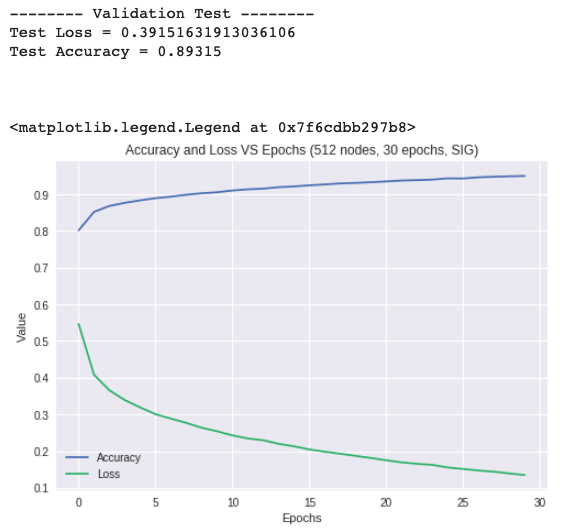
\includegraphics[scale = 0.3]{512_SIG.png}
        \caption{512 Neurons and Sigmoid}
    \end{figure}

    Overall the sigmoid function performed best as the activation function of the hidden layer. It was much faster at reaching the lowest error value.

    \subsection{A6: Retraining Network}

    Here we retrain the network with 512 nodes, 30 epochs and the sigmoid activation for hidden layer. The network was trained for 60000 images and the tested on the 20000 test data. The code is in the jupyter notebooks final cell.

    \begin{figure}[h!]
        \centering
        \captionsetup{justification=centering}
        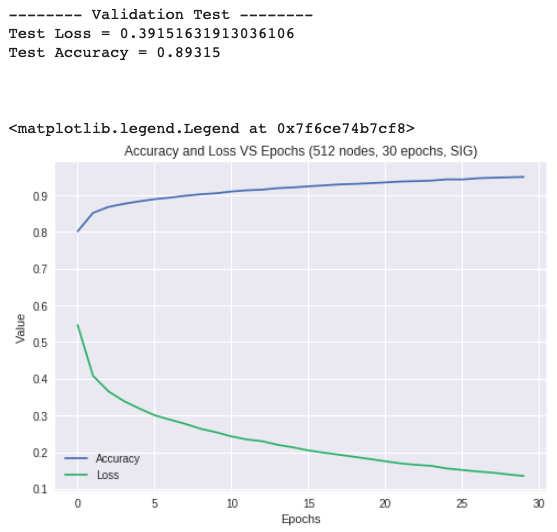
\includegraphics[scale = 0.4]{Final.png}
        \caption{Network trained on all training data and then tested on testing data}
    \end{figure}

    This network had the best performance on all previously trained networks and the confusion matrix for it is shown below:

    \begin{figure}[h!]
        \centering
        \captionsetup{justification=centering}
        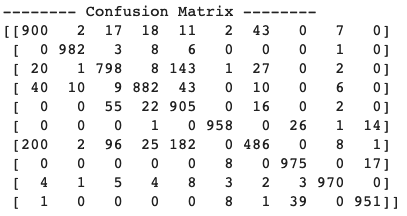
\includegraphics[scale = 0.4]{cm.png}
        \caption{Confusion Matrix}
    \end{figure}

    \section{Task 3: Theory Questions}

    \subsection{Q1}

    What is generalization in the context of machine learning. Is it better for the machine learning algorithms to generalize?

    \subsection{A1}

    Generalization is the ability for a network to figure out/adapt to the new input data. It determines how well a network will perform on data it has never seen before. Generalization is better because the better the network is at it, the better it will be with brand new data. If a system does not generalize then it will be unable to adapt.

    \subsection{Q2}

    What is overfitting and under-fitting, how is it related to generalization?
    
    \subsection{A2}

    Overfitting is when the network essentially 'memorizes' the data and it manages to lower it's cost function heavily however this sort of behavior means it is unable to generalize and it will do well on training data but not on real life data.
    Under-fitting is when the network is unsuccesfully trained and it's cost function is not as low as it can get, this means that it performs poorly on training data as well as test data. It's weights need to be adjusted further. 

    \subsection{Q3}

    What is capacity of a neural network? Is it related to generalization, if so how?

    \subsection{A3}

    Capacity of a network is how much the network is able to learn. The more it is able to learn the more complex it's model will become. In relation to generalization, a network that is extremely complex can tend to overfit on a very simple problem, however, on a complex problem it will be good at picking up the subtle nuances of the input data. So a network with low capacity can underfit while a network with high capacity can often overfit. It is vital to find a middle ground

    \subsection{Q4}

    What is the relationship between number of epochs and overfitting?

    \subsection{A4}

    If the number of epochs (iterations) exceeds a certain value the model can start to overfit the data. Initially the increasing number of epochs can improve accuracy but after a limit the network starts overfitting

    \subsection{Q5}

    What is weight regularization? How does it improve generalizations? Write a code snippet that can be included in Task 2 for adding weight regularization.

    \subsection{A5}

    When the weights of a network tend to increase by a large amount we reduce them through normalization techniques. This is called weight regularization and it is used to reduce the chances of overfitting in a network. This is because in a network with overfitting there are usually large weights so by making them smaller and reducing them through normalization we tend to prevent overfitting. This in turn helps the network generalize better. Below is some code that shows how we would implement regularization on the Fashion MNIST code

    \begin{lstlisting}[language=python, caption=Network with Weight Regularization]
    import keras
    from keras.models import Sequential
    from keras.layers import Dense
    from keras import regularizers
    
    model = Sequential()

    model.add(Dense(16,
                    input_dim=784,
                    kernel_regularizer=regularizers.l2(0.01),
                    activity_regularizer=regularizers.l1(0.01)))

    model.add(Dense(10,
                    activation='softmax',
                    kernel_regularizer=regularizers.l2(0.01),
                    activity_regularizer=regularizers.l1(0.01)))

    model.compile(optimizer='rmsprop',
                  loss='categorical_crossentropy',
                  metrics=['accuracy'])\end{lstlisting}

    \subsection{Q6}

    What is drop out? How does it improve generalizations? Write a code snippet that can be included in Task 2 for adding drop out.

    \subsection{A6}

    Dropout is when we randomly turn some of the weights in the network to 0, thereby forcing the network to learn based on other parameters. This reduces dependency on a single weight and it also helps prevent overfitting.

    \begin{lstlisting}[language=python, caption=Network with Dropout]
    import keras
    from keras.models import Sequential
    from keras.layers import Dense
    from keras.layers import Dropout

    model = Sequential()
    
    model.add(Dropout(0.2))

    model.add(Dense(16, input_dim=784,))

    model.add(Dropout(0.2))

    model.add(Dense(10, activation='softmax',))

    model.compile(optimizer='rmsprop',
                  loss='categorical_crossentropy',
                  metrics=['accuracy'])\end{lstlisting}

    \pagebreak

    \begin{thebibliography}{9}
        \bibitem{notes} 
        Usman Tariq Notes and Slides from ELE494. 
        
        \bibitem{eli} 
        Eli Bendersky's Website. 
        \textit{The Softmax Function and its derivative}
        \\\texttt{https://eli.thegreenplace.net/2016/the-softmax-function-and-its-derivative/}
        
        \bibitem{kerasdocs} 
        Keras Documentation,
        \\\texttt{https://keras.io/}
    \end{thebibliography}
\end{document} 